% !TEX TS-program = pdflatex
% !TEX encoding = UTF-8 Unicode

% This is a simple template for a LaTeX document using the "article" class.
% See "book", "report", "letter" for other types of document.

\documentclass[11pt]{article} % use larger type; default would be 10pt

\usepackage[utf8]{inputenc} % set input encoding (not needed with XeLaTeX)

%%% Examples of Article customizations
% These packages are optional, depending whether you want the features they provide.
% See the LaTeX Companion or other references for full information.

%%% PAGE DIMENSIONS
\usepackage[a4paper,left=2cm,right=2cm,top=2cm,bottom=2cm]{geometry}
%\usepackage{geometry} % to change the page dimensions
% \geometry{a4paper} % or letterpaper (US) or a5paper or....
% \geometry{margin=0in} % for example, change the margins to 2 inches all round
% \geometry{landscape} % set up the page for landscape
%   read geometry.pdf for detailed page layout information

\usepackage{graphicx} % support the \includegraphics command and options

\usepackage[parfill]{parskip} % Activate to begin paragraphs with an empty line rather than an indent

%%% PACKAGES
\usepackage{booktabs} % for much better looking tables
\usepackage{array} % for better arrays (eg matrices) in maths
\usepackage{paralist} % very flexible & customisable lists (eg. enumerate/itemize, etc.)
\usepackage{verbatim} % adds environment for commenting out blocks of text & for better verbatim
\usepackage{subfig} % make it possible to include more than one captioned figure/table in a single float
\usepackage{amsmath}
\usepackage{amssymb}
\usepackage{logicproof}
\usepackage{tikz}
\usepackage{hyperref}
\usetikzlibrary{arrows,petri,topaths}
\usepackage{float}
\usepackage{graphicx}
\usepackage[T1]{fontenc}
\usepackage{listings}
\lstset{
  basicstyle=\ttfamily,
  mathescape
}
% These packages are all incorporated in the memoir class to one degree or another...

%%% HEADERS & FOOTERS
\usepackage{fancyhdr} % This should be set AFTER setting up the page geometry
\pagestyle{fancy} % options: empty , plain , fancy
\renewcommand{\headrulewidth}{0pt} % customise the layout...
\lhead{}\chead{}\rhead{}
\lfoot{}\cfoot{\sffamily\thepage\normalfont}\rfoot{}

%%% SECTION TITLE APPEARANCE
\usepackage{sectsty}
\allsectionsfont{\sffamily\mdseries\upshape} % (See the fntguide.pdf for font help)
% (This matches ConTeXt defaults)

%%% ToC (table of contents) APPEARANCE
\usepackage[nottoc,notlof,notlot]{tocbibind} % Put the bibliography in the ToC
\usepackage[titles,subfigure]{tocloft} % Alter the style of the Table of Contents
\renewcommand{\cftsecfont}{\rmfamily\mdseries\upshape}
\renewcommand{\cftsecpagefont}{\rmfamily\mdseries\upshape} % No bold!
\newcommand{\qedsymbol}{\rightline{$\blacksquare$}}
\renewcommand{\familydefault}{\sfdefault}
\renewcommand{\thesection}{\hspace{-0.5cm}\arabic{section}}
\renewcommand{\thesubsection}{\alph{subsection})}

\usepackage[style=numeric-comp]{biblatex}

%%% END Article customizations

%%% The "real" document content comes below...

\title{\vspace{-1.6cm}Bioinformatics Assignment}
\author{zrlr73}
\date{} % Activate to display a given date or no date (if empty),
         % otherwise the current date is printed 

\begin{document}
\maketitle

\section{Markov Models}
\subsection{HMMs with silent states}
Since the Viterbi algorithm is already popular for solving this problem without silent states, I decided to adapt it forthe inclusion of silent states. The Viterbi algorithm iterates using the observed output of the modelled HMM, constructing a trellis of possible states for each observed output. Since we need to cater for states that do not provide any output whatsoever, we need to be able to generate possible silent states as well as the existing trellis of non-silent states. We also need to consider these silent states alongside the non-silent ones when deciding on possible precursors for each observed outcome.

Therefore, I would propose the following modified Viterbi algorithm:
\begin{lstlisting}
Initialise trellis with $v_0(0)=1, v_k(0)=0\quad|\quad k>0$
Initialise 2D array of linked list heads with size $m\times L$

// For each observed output
For $i=1\text{ to }L$ do:
  // For each possible state
  For each state $l$ do:
    $v_l(i) = e_l(x_i) \times max_k\{v_k(i-1)\times m_{kl}\}$

  // Evaluate possible silent states
  Initialise array $a$ of linked list heads with length $m$ and $a_0=v_l$
  Initialise numeric array $b$ with length $m$
  Integer j = 0
  Initialise Boolean value $loop$
  Do:
    j++
    loop = false
    For each state $s$ do:
      $a_j(s) = e_s($silent$)\times max_f\{a_{j-1}(f)\times m_{fs}\}$

      if ($a_j(s) > v_l(s)$ and $a_j(s) > a_{j-1}(s)$):
        loop = true
  While (loop)

\end{lstlisting}

\subsection{The Expectation-Maximisation Algorithm}
bruh



\section{Tree Reconstruction}

\subsection{The BUILD Algorithm}
If we call $(i,j)$ the lowest common ancestor of the leaves $i$ and $j$ of a tree, we can also define an operator $<$ which denotes the hierarchy of lowest common ancestors. For example, the constraint $(i,j)<(k,l)$ tells us that the lowest common ancestor of $k$ and $l$ is itself an ancestor of the lowest common ancestor of $i$ and $j$ - see figure below.

\begin{figure}
	\centering
	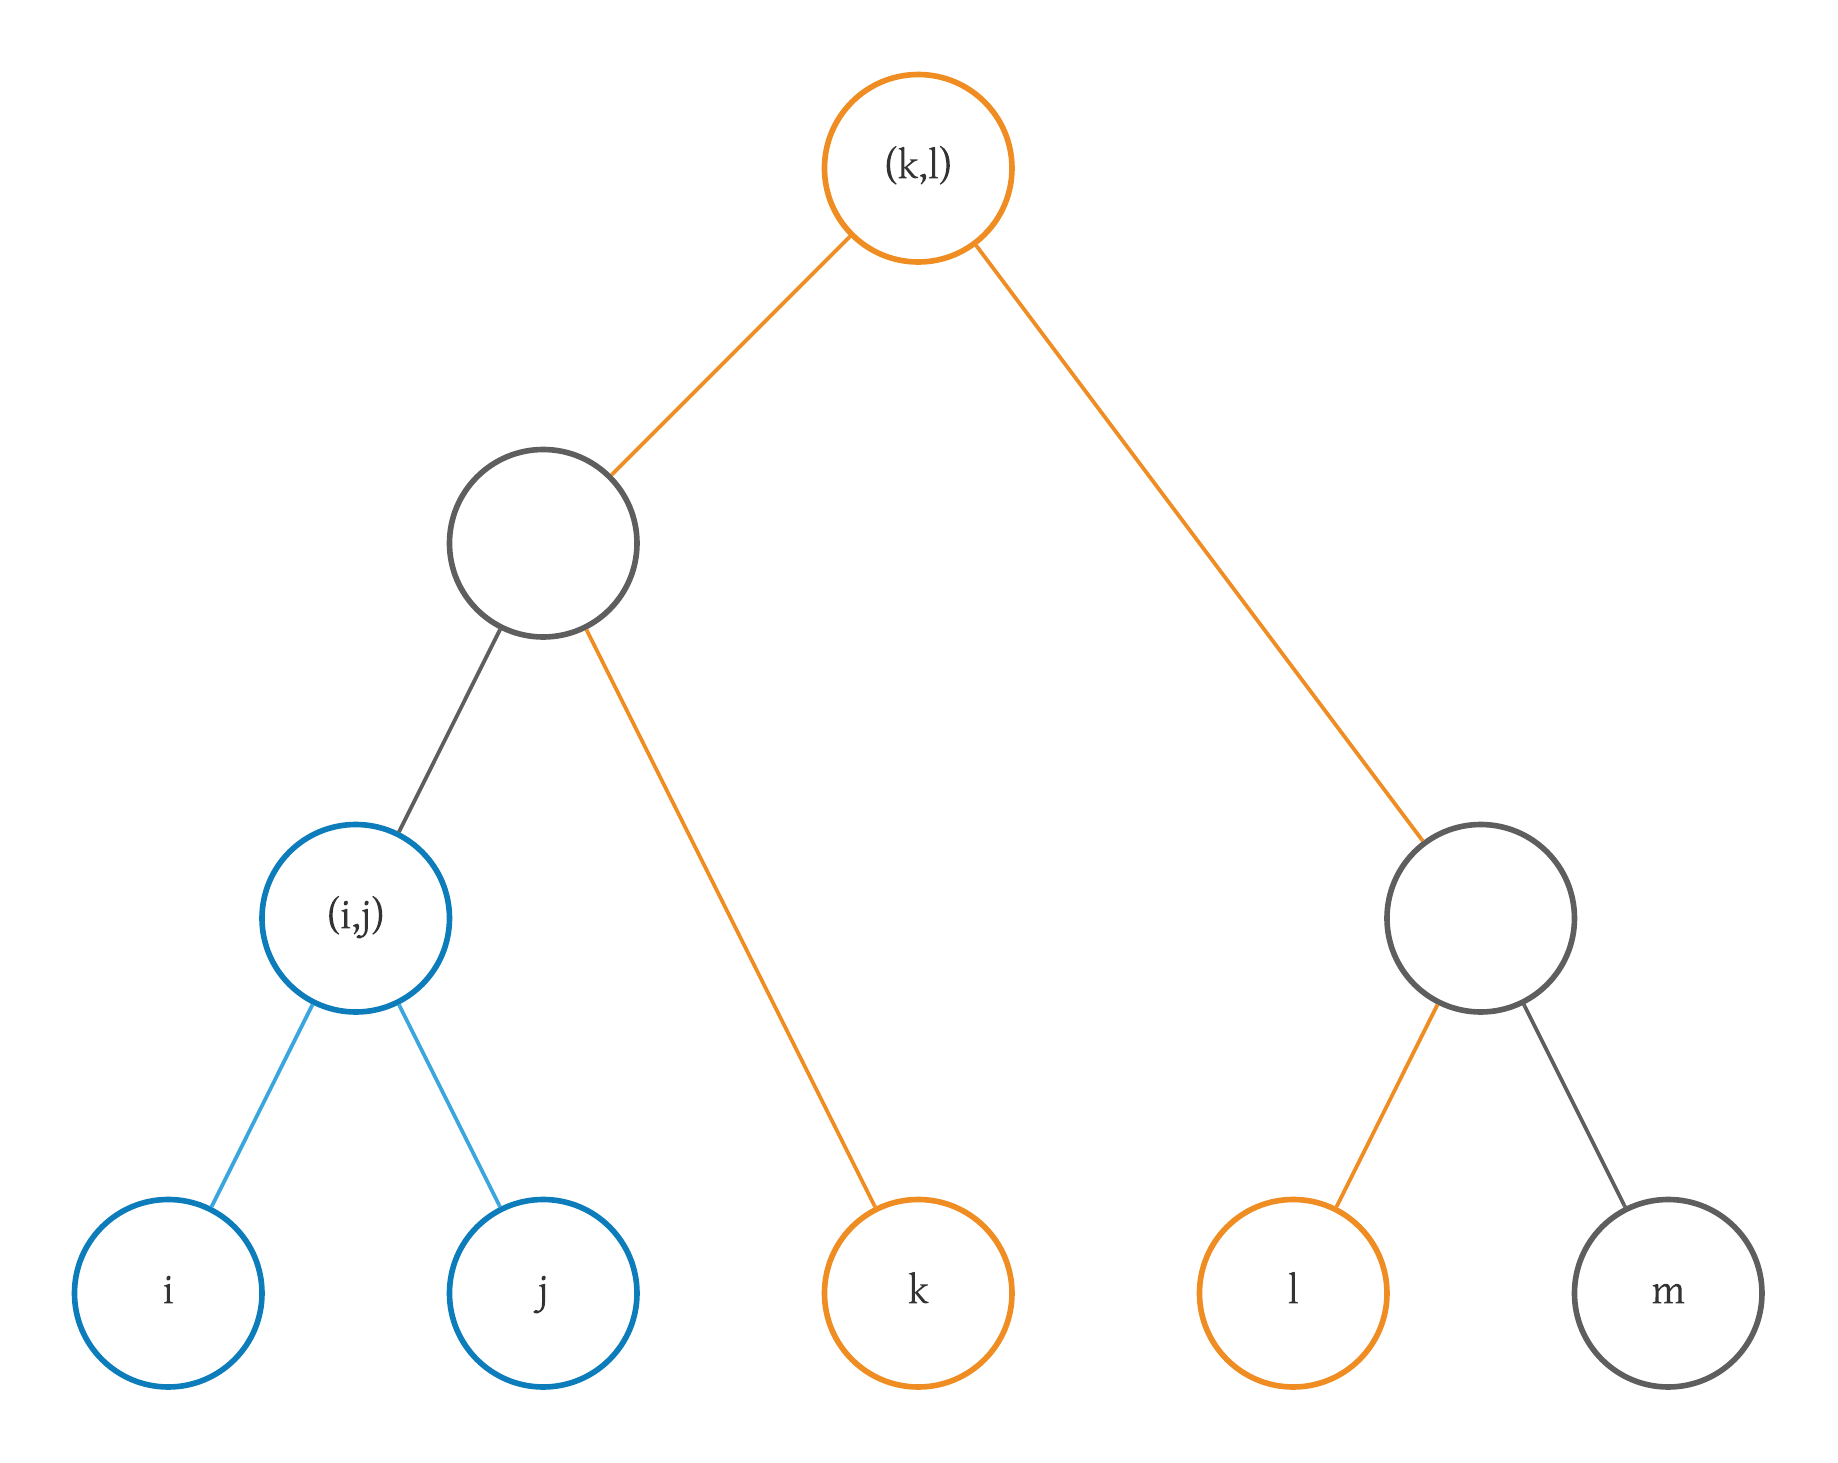
\includegraphics[width=10cm]{buildtree}
\end{figure}

The purpose of the BUILD algorithm is to construct a tree solely from these constraints. In a bioinformatics context, assuming the tree is a phylogeny, the constraints would be describing how closely related pairs of species are. As an example, we would specify the above constraint if we knew that the four species $\{i,j,k,l\}$ all had a common ancestor, but $i$ and $j$ were more closely related to each other than to the rest.

In BUILD, the structure of a tree is inferred using a technique known as 'partitioning'. This is when the set of leaves is split into groups known as 'blocks' at the root - for example, assuming descriptive enough constraints, the above tree would be split into the two sets $\{i,j,k\}$ and $\{l,m\}$. This partitioning can be done fairly easily using logical properties of the constraints:

From any constraint $(i,j)<(k,l)$ we can infer that:
\begin{enumerate}
	\item $i$ and $j$ are in the same block.
	\item If we already know that $k$ and $l$ are in the same block, then $i$ and $j$ must also be in that same block.
\end{enumerate}

We also assume that no two leaves are in the same block unless we can infer that they are from the constraints. In the original paper, this is the third rule.

With the set of leaves split into at least two blocks, we recurse into each block, partitioning every block until there is only one leaf left in the set. At this point, the algorithm's recursive structure exactly reflects the tree being constructed, so it simply needs to construct and return a tree. Instances with just one leaf return it, and instances that partitioned items join the returned structures with a new node until the outer layer is reached and the tree is complete.


\subsection{Partitioning}
Partitioning could occur as follows:
\begin{lstlisting}
// a 2D array: items in this array will be referred to as 'blocks'
$\pi_C$ = []

For each constraint $(a,b)<(c,d)$:
  If neither $a$ nor $b$ already exists in $\pi_C$:
    Add the new block [$a$,$b$] to $\pi_C$

  Else if $a$ and $b$ already exist in separate blocks in $\pi_C$:
    Replace those two blocks with their union

  Else if $a$ already exists in a block in $\pi_C$:
    Add $b$ to that block
  Else if $b$ already exists in a block in $\pi_C$:
    Add $a$ to that block

For each constraint $(a,b)<(c,d)$:
  If $c$ and $d$ share a block, merge the block containing $a$ and $b$ into it

For each leaf $x$ that is not a member of an existing block:
  Add the new block [$x$] to $\pi_C$
\end{lstlisting}

The result of this algorithm is the 2D array $\pi_C$, with structure as follows:
\begin{lstlisting}
[
  [i, j, k],
  [l, m, o],
  [n]
]
\end{lstlisting}
Each sub-array corresponds to a block $S_i$, with letters denoting the leaves in that block.


\subsection{Example}


\subsection{Reversing BUILD}


\end{document}
